\chapter{带宽自适应的通信数据压缩}
\section{引言}
在分布式深度学习中，减少通信数据量是降低通信开销最直接的方式，可以在参数同步拓扑优化的基础上进一步减少通信时间，提高训练效率。目前用于减少通信数据量的主要手段是通信数据压缩，包括量化和稀疏化。由于数据压缩往往是有损压缩，会导致信息量的丢失，从而不可避免地影响模型精度，并且压缩程度越高，对模型精度的影响越大，甚至可能会导致模型无法收敛。为了降低压缩对模型精度的影响，一些现有的方法引入了差分压缩和压缩误差补偿等策略，然而压缩程度过高时模型精度还是会有所下降。另外现有的方法对不同节点采用相同的压缩程度，这使得在带宽异构场景下进行同步训练时，带宽不同的链路上通信时间不同，从而导致通信带宽较大的链路利用率较低，造成资源的浪费。

针对上述问题，本章提出了带宽自适应的量化分布式随机梯度下降算法（BA-QDSG D）和带宽自适应的量化分布式随机梯度跟踪算法（BA-QDSGT）。首先，基于差分压缩和压缩误差补偿实现量化分布式随机梯度下降算法和量化分布式随机梯度跟踪算法。然后在此基础上引入带宽自适应策略，根据带宽矩阵调整每条边上通信数据的压缩程度，以降低某些带宽较高的边上的数据压缩误差，提高模型精度，同时提高通信资源的利用率。最后在Cifar10数据集上进行分布式深度学习实验，验证了本章提出的带宽自适应的通信数据压缩方法的有效性。

本章其他小结的内容安排如下：4.2节介绍了分布式深度学习中两种经典的基于去中心化架构的算法，分布式随机梯度下降算法（DSGD）和分布式随机梯度跟踪算法（DSGT）；4.3节介绍了本章采用的量化策略并提出了带宽自适应的量化分布式训练算法；4.4节基于Cifar10数据集上的分布式深度学习实验对提出的算法进行验证分析；4.5节对本章内容进行了总结。

\section{分布式训练算法}
\subsection{分布式随机梯度下降算法} \label{subsection-4-2-1}
分布式随机梯度下降算法（Distributed Stochastic Gradient Descent，简称DSGD）是最早提出的基于去中心化的分布式（Gossip）架构的优化算法，该算法是随机梯度下降算法（Stochastic Gradient Descent，简称SGD）的一种变体，旨在通过将计算任务分布到多个计算节点或设备上来提高训练效率。在该算法中，节点只对参数进行通信，并利用本地随机梯度对融合后的参数进行更新。正是由于该算法原理简单，并且拥有可以媲美集中式算法的性能而被广泛研究。

DSGD算法的实现过程可以简单地描述为三个步骤：1）随机采样本地数据计算梯度；2）通信并融合模型参数；3）本地随机梯度搜索。其中本地随机梯度搜索是在模型参数融合之后进行的，当然也可以在模型参数融合之前进行本地随机梯度搜索，本章仅研究前一种算法实现。根据上述实现过程，DSGD算法的原理可以表示为如下形式：
\begin{equation}
    \label{tab:DSGD-equation}
    \begin{aligned}
        \boldsymbol{x}_{k+1} =W\boldsymbol{x}_k -\gamma \nabla f\left( \boldsymbol{x}_k \right),
    \end{aligned}
\end{equation}
其中$\boldsymbol{x}_k =\left( \boldsymbol{x}_{1,k} ,...,\boldsymbol{x}_{n,k} \right) ^T$，$\nabla f\left( \boldsymbol{x}_k \right) =\left( \nabla f_1\left( \boldsymbol{x}_{1,k} \right) ,...,\nabla f_n\left( \boldsymbol{x}_{n,k} \right) \right) ^T$，$\boldsymbol{x}_{i,k} $是节点$i$在第$k$次迭代的模型参数，$f_i\left( \cdot \right) $是节点$i$的本地损失函数，$\nabla f_i\left( \boldsymbol{x}_{i,k} \right) $是节点$i$在第$k$次迭代的本地随机梯度，$W\in \mathbb{R} ^{n\times n}$是权重矩阵，$\gamma$是步长。

由于Gossip架构的拓扑结构的约束，网络中的每个节点仅有本地数据以及部分邻居的信息，因此需要一个有效的通信机制来保障节点的本地信息能够在整个网络中流通，从而使各节点的模型参数最终收敛到一致。在DSGD算法中，通过令权重矩阵$W$满足\autoref{section3-2-1}中描述的条件即可实现模型参数的一致性。另外，与\autoref{section3-2-1}中介绍的线性平均一致问题的迭代过程相比，DSGD增加了一个本地随机梯度搜索项，即$\nabla f\left( \boldsymbol{x}_k \right)$，该步骤推动模型参数朝最优值更新，所以DSGD算法能够使得各节点的模型参数收敛到一致的最优解。

基于以上介绍，DSGD算法的伪代码如下：
\begin{center}
    % \begin{minipage}{8.5cm}
    \begin{algorithm}[!htbp]
            \caption{节点$i$上的DSGD算法} 
        %   \small
            \label{Algorithm-DSGD} 
            \begin{algorithmic}[1]
            \REQUIRE{模型参数初始值$\boldsymbol{x}_{i,0}$，步长$\gamma$，权重矩阵$W$，迭代次数$K$}；
            \ENSURE{所有节点模型参数的平均值$\frac{1}{n}\sum_{i=1}^n{\boldsymbol{x}_{i,K}}$}；
            \FOR{$k=0,1,...,K-1$}
                \STATE 从节点$i$的本地数据集中随机采样数据$\xi _{i,k} $；
                \STATE 计算本地随机梯度：$\nabla f_i\left( \boldsymbol{x}_{i,k} \right) =\nabla f_i\left( \boldsymbol{x}_{i,k},\xi _{i,k} \right) $；
                \STATE 与邻居节点通信，并利用本地模型参数和接收到的参数计算加权平均值：$\boldsymbol{x}_{i,k+\frac{1}{2}}=\sum_{j=1}^n{W_{ij}\boldsymbol{x}_{j,k}}$；
                % \begin{align*}
                %     \boldsymbol{x}_{i,k+\frac{1}{2}}=\sum_{j=1}^n{W_{ij}\boldsymbol{x}_{j,k}};
                % \end{align*}
                \STATE 更新本地模型参数：$\boldsymbol{x}_{i,k+1}=\boldsymbol{x}_{i,k+\frac{1}{2}}-\gamma \nabla f_i\left( \boldsymbol{x}_{i,k} \right) $。
            \ENDFOR            
            \end{algorithmic}
    \end{algorithm}
    % \end{minipage}
\end{center}

% \vspace{-5pt}
\subsection{分布式随机梯度跟踪算法}
虽然DSGD算法能够使得各节点的模型参数收敛到一致，但是由于各节点的本地数据集不同，因此在进行本地随机梯度搜索后，节点模型参数又将变得不一致。为了减小节点本地随机梯度搜索对一致性的影响，通常需要采用衰减的步长，即随着迭代次数的增加，步长逐渐趋向于零，对应算法中的$\nabla f\left( \boldsymbol{x}_k \right)$逐渐趋向于零，这必然会导致模型的收敛速度变慢。为了解决这一问题，分布式随机梯度跟踪算法（Distributed Stochastic Gradient Tracking，简称DSGT）被提了出来。该算法允许使用恒定的步长进行训练，同时能够保证各节点的模型参数收敛到一致的最优解。

DSGT算法与DSGD算法的主要不同在于DSGT算法对每个节点引入了一个辅助变量用于跟踪所有节点本地目标函数的平均梯度，并且在训练过程中，不仅对模型参数进行通信和融合，也对该辅助变量进行通信和融合，然后使用该辅助变量代替随机梯度对本地模型参数进行更新。DSGT算法的原理可以表示为如下形式：
\begin{equation}
    \label{tab:DSGT-equation}
    \begin{aligned}
        \boldsymbol{x}_{k+1}&=W\boldsymbol{x}_k-\gamma \boldsymbol{y}_k,
        \\
        \boldsymbol{y}_{k+1}&=W\boldsymbol{y}_k+\nabla f\left( \boldsymbol{x}_{k+1} \right) -\nabla f\left( \boldsymbol{x}_k \right),
    \end{aligned}
\end{equation}
其中$\boldsymbol{y}_k=\left( \boldsymbol{y}_{1,k},...,\boldsymbol{y}_{n,k} \right) ^T$，$\boldsymbol{y}_{i,k}$是节点$i$用于跟踪平均梯度的辅助变量，其他变量的含义与\autoref{tab:DSGD-equation}中变量的含义相同。

在每次迭代中，节点之间利用参数同步拓扑进行模型参数和辅助变量的融合，并且为了实现一致性，权重矩阵$W$同样需要满足\autoref{section3-2-1}中描述的条件。下面说明DSGT算法实现梯度跟踪的原理：

由于权重矩阵$W$是双随机矩阵，则对\autoref{tab:DSGT-equation}的第二个等式两边同时左乘$\mathbf{1}^T$后，根据$\boldsymbol{y}_0=\nabla f\left( \boldsymbol{x}_0 \right)$，可以得到：
\begin{equation}
    \label{tab:equ-4-3}
    \begin{aligned}
        \mathbf{1}^T\boldsymbol{y}_{k+1}&=\mathbf{1}^T\boldsymbol{y}_k+\mathbf{1}^T\nabla f\left( \boldsymbol{x}_{k+1} \right) -\mathbf{1}^T\nabla f\left( \boldsymbol{x}_k \right) 
        \\
        &=\mathbf{1}^T\nabla f\left( \boldsymbol{x}_{k+1} \right) .
    \end{aligned}
\end{equation}
然后由DSGT算法的一致性，每个节点的辅助变量最终收敛到相同的值，则有：
\begin{equation}
    \label{tab:equ-4-4}
    \boldsymbol{y}_{i,k}=\frac{1}{n}\mathbf{1}^T\nabla f\left( \boldsymbol{x}_k \right) ,\  i=1,...,n,
\end{equation}
从而实现对全局平均梯度的跟踪。因此，随着迭代次数的增加，每个节点的本地模型参数最终将朝着相同的方向更新，并且当算法收敛时，节点参数达到最优值$\boldsymbol{x}^*$，平均梯度$\mathbf{1}^T\nabla f\left( \boldsymbol{x}^* \right) =\mathbf{0}$。

根据以上分析，DSGT算法通过引入辅助变量实现了梯度跟踪，避免了节点本地梯度搜索对一致性的影响，因此可以使用恒定的步长，从而保证了算法的收敛速度。DSGT算法的伪代码如下：
% \vspace{-15pt}
\begin{center}
    % \begin{minipage}{8.5cm}
    \begin{algorithm}[!htbp]
            \caption{节点$i$上的DSGT算法} 
        %   \small
            \label{Algorithm-DSGT} 
            \begin{algorithmic}[1]
            \REQUIRE{模型参数初始值$\boldsymbol{x}_{i,0}$，辅助变量初始值$\boldsymbol{y}_{i,0}=\nabla f_i\left( \boldsymbol{x}_{i,0} \right) $，步长$\gamma$，权重矩阵$W$，迭代次数$K$}；
            \ENSURE{所有节点模型参数的平均值$\frac{1}{n}\sum_{i=1}^n{\boldsymbol{x}_{i,K}}$}；
            \FOR{$k=0,1,...,K-1$}
                \STATE 与邻居节点通信模型参数，并利用本地模型参数和接收到的参数计算加权平均值：$\boldsymbol{x}_{i,k+\frac{1}{2}}=\sum_{j=1}^n{W_{ij}\boldsymbol{x}_{j,k}}$；
                % \begin{align*}
                %     \boldsymbol{x}_{i,k+\frac{1}{2}}=\sum_{j=1}^n{W_{ij}\boldsymbol{x}_{j,k}};
                % \end{align*}
                \STATE 利用辅助变量$\boldsymbol{y}_{i,k}$更新本地模型参数：$\boldsymbol{x}_{i,k+1}=\boldsymbol{x}_{i,k+\frac{1}{2}}-\gamma \boldsymbol{y}_{i,k}$；
                \STATE 与邻居节点通信辅助变量，并利用本地辅助变量和接收到的辅助变量计算加权平均值：$\boldsymbol{y}_{i,k+\frac{1}{2}}=\sum_{j=1}^n{W_{ij}\boldsymbol{y}_{j,k}}$；
                % \begin{align*}
                %     \boldsymbol{y}_{i,k+\frac{1}{2}}=\sum_{j=1}^n{W_{ij}\boldsymbol{y}_{j,k}};
                % \end{align*}
                \STATE 从节点$i$的本地数据集中随机采样数据$\xi _{i,k+1} $；
                \STATE 计算本地随机梯度：$\nabla f_i\left( \boldsymbol{x}_{i,k+1} \right) =\nabla f_i\left( \boldsymbol{x}_{i,k+1},\xi _{i,k+1} \right) $；
                \STATE 更新辅助变量：$\boldsymbol{y}_{i,k+1}=\boldsymbol{y}_{i,k+\frac{1}{2}}+\nabla f_i\left( \boldsymbol{x}_{i,k+1} \right) -\nabla f_i\left( \boldsymbol{x}_{i,k} \right) $。
            \ENDFOR            
            \end{algorithmic}
    \end{algorithm}
    % \end{minipage}
\end{center}


\section{带宽自适应的量化分布式训练算法}
本节在DSGD算法和DSGT算法的基础上提出了带宽自适应的量化分布式随机梯度下降算法（Bandwidth Adaptive Quantized Distributed Stochastic Gradient Descent，简称BA-QDSGD）和带宽自适应的量化分布式随机梯度跟踪算法（Bandwidth Adaptive Quantized Distributed Stochastic Gradient Tracking，简称BA-QDSGT）。首先将介绍本节使用的量化策略，然后介绍基于差分压缩和压缩误差补偿的量化算法，并在此基础上引入带宽自适应策略，设计带宽自适应的量化算法。

\subsection{量化策略设计}
在分布式深度学习中，通常使用32比特浮点数来表示模型的参数和梯度，量化是在节点之间通信模型参数或梯度之前将待通信的数据压缩至更低的比特数，从而减少通信的数据量。对于任意一个32比特的浮点数向量$\boldsymbol{v}\in \mathbb{R} ^d$，本节使用下式对其每一维度的元素$v_i$进行量化：
\begin{equation}
    \label{tab:equ-4-5}
    Q_{\ell}\left( v_i \right) =\left\| \boldsymbol{v} \right\| _{\infty}\cdot \mathrm{sign}\left( v_i \right) \cdot \varphi _i(\boldsymbol{v},\ell ).
\end{equation}
其中$\left\| \boldsymbol{v} \right\| _{\infty}$是向量$\boldsymbol{v}$的无穷范数，$\mathrm{sign}\left( \cdot \right) $是符号函数，$\varphi _i(\boldsymbol{v},\ell )$是如下定义的独立随机变量：
\begin{equation}
    \label{tab:equ-4-6}
    \varphi _i(\boldsymbol{v},\ell )=\begin{cases}
        \frac{s}{\ell}&		\,\,\mathrm{with}\  \mathrm{probability}\  1+s-\frac{\left| v_i \right|}{\left\| \boldsymbol{v}_{\infty} \right\|}\ell\\
        \frac{s+1}{\ell}&		\,\,\mathrm{otherwise}\\
    \end{cases},
\end{equation}
其中$s$为满足$0\leqslant s<\ell $的整数，并且$\frac{v_i}{\left\| \boldsymbol{v} \right\| _{\infty}}\in \left[ \frac{s}{\ell},\frac{s+1}{\ell} \right] $，$\ell$一般定义为$2^{\mathrm{b}-1}$，表明使用该量化方法后，向量的每一维度只需要使用$\mathrm{b}$个比特就可以表示。因此$\mathrm{b}$的值衡量了量化的程度，$\mathrm{b}$越小则说明量化的程度越高，相应的量化精度越低。

在使用\autoref{tab:equ-4-5}对向量进行量化后，可以得到：
\begin{equation}
    \label{tab:equ-4-7}
    \begin{aligned}
        E\left[ Q_{\ell}\left( v_i \right) \right] &=\left\| \boldsymbol{v} \right\| _{\infty}\cdot \mathrm{sign}\left( v_i \right) \left[ \frac{s}{\ell}\times \left( 1+s-\frac{\left| v_i \right|}{\left\| \boldsymbol{v} \right\| _{\infty}}\ell \right) +\frac{s+1}{\ell}\left( \frac{\left| v_i \right|}{\left\| \boldsymbol{v} \right\| _{\infty}}\ell -s \right) \right]\\
        &=\left\| \boldsymbol{v} \right\| _{\infty}\cdot \mathrm{sign}\left( v_i \right) \frac{v_i}{\left\| \boldsymbol{v} \right\| _{\infty}}\\
        &=v_i\\
    \end{aligned}.
\end{equation}
该式说明量化后向量中每一维度的元素的期望等于原向量对应位置元素的值，并且Liu等人\cite{liu2020linear}证明了该量化策略可以保证量化后的向量与原向量距离的方差是有界的，因此在一定量化程度下该量化策略可以保持分布式深度学习算法的收敛性。

进一步地，为了便于通信，将\autoref{tab:equ-4-5}改写为如下形式：
\begin{equation}
    \label{tab:equ-4-8}
    Q_{\ell}\left( \boldsymbol{v} \right) =\frac{\left\| \boldsymbol{v} \right\| _{\infty}}{2^{\mathrm{b}-1}}\cdot \mathrm{sign}\left( \boldsymbol{v} \right) \odot \lfloor \frac{2^{\mathrm{b}-1}\left| \boldsymbol{v} \right|}{\left\| \boldsymbol{v} \right\| _{\infty}}+\boldsymbol{w} \rfloor ,
\end{equation}
其中$\odot$为哈达玛积，$\lfloor \cdot \rfloor $表示对元素向下取整，$\boldsymbol{w}\in \mathbb{R} ^d$是扰动向量，其每一维度的元素符合如下分布：
\begin{equation}
    \label{tab:equ-4-9}
    w_i=\begin{cases}
        0&		\,\,\mathrm{with} \mathrm{probability} 1+s-\frac{\left| v_i \right|}{\left\| \boldsymbol{v}_{\infty} \right\|}\ell\\
        1&		\,\,\mathrm{otherwise}\\
    \end{cases}.
\end{equation}

然后，在每次通信时可以将量化后的向量分为幅值、符号向量和整数向量三部分进行通信，其中幅值$\frac{\left\| \boldsymbol{v} \right\| _{\infty}}{2^{b-1}}$为浮点数标量，符号向量$\mathrm{sign}\left( \boldsymbol{v} \right)$中的元素为±1和0，该部分表示为8比特整数向量，整数向量$\lfloor \frac{2^{\mathrm{b}-1}\left| \boldsymbol{v} \right|}{\left\| \boldsymbol{v} \right\| _{\infty}}+\boldsymbol{w} \rfloor$中的元素为小于$2^\mathrm{b}$的整数，该部分在$\mathrm{b}=16$时表示为16比特整数向量，在$\mathrm{b}=1/2/4/8$时表示为8比特整数向量。

%接下来介绍转换方法，添加一张图
对于符号向量和$\mathrm{b}=1/2/4$时的整数向量，为了降低通信开销，将多个元素组合成一个8比特的整数进行通信。下面以$\mathrm{b}=4$为例进行说明，如\autoref{fig:Fig4-1}所示，向量$\boldsymbol{v}$被量化为4比特整数向量后，每两个元素一组将4比特整数向量拼接为新的8比特整数向量，然后对该向量进行通信，并在接收到数据后，通过整除和取余操作将数据还原成原来的4比特向量。其中，拼接操作通过下式实现：
\begin{equation}
    \label{tab:equ-4-10}
    v^{_{8bit}}=16\times v_{1}^{4bit}+v_{2}^{4bit}.
\end{equation}
还原操作通过下式实现：
\begin{equation}
    \label{tab:equ-4-11}
    \begin{aligned}
        v_{1}^{4bit}=\lfloor \frac{v^{_{8bit}}}{16} \rfloor 
    \\
    v_{2}^{4bit}=v^{_{8bit}}\%16.
    \end{aligned}
\end{equation}

\begin{figure}[!htbp]   
    \centering
    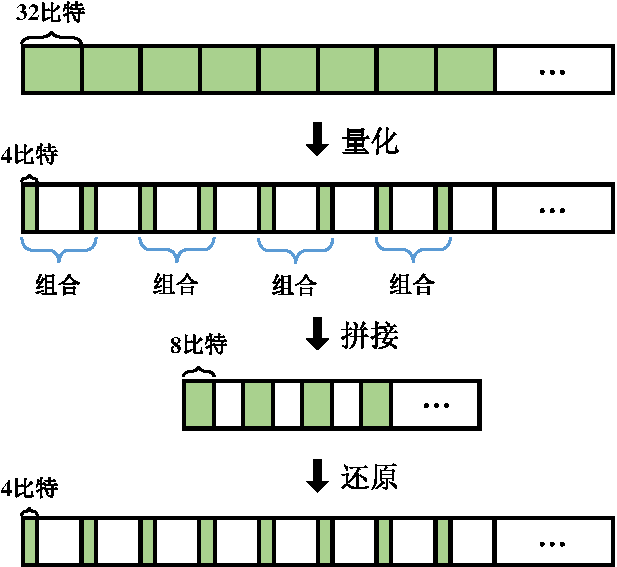
\includegraphics[width=0.5\linewidth]{figure/chapter4/fig4-1-quantize.pdf}
    \caption{\label{fig:Fig4-1}数据量化流程}
\end{figure}

\subsection{带宽自适应的量化分布式训练算法设计}
本小节通过对DSGD算法和DSGT算法引入差分压缩和压缩误差补偿实现量化分布式随机梯度下降算法和量化分布式随机梯度跟踪算法的设计，设计过程如\autoref{fig:Fig4-2}所示。首先，对模型参数/梯度引入对应的状态变量。然后使用上一小节中介绍的量化策略对模型参数/梯度与状态变量的差进行压缩，这一步则是差分压缩。接下来将状态变量与量化后的值求和得到对模型参数/梯度的估计值，该估计值被用于节点与邻居节点间的通信。模型参数/梯度与该估计值的差可以看作是差分压缩导致的误差，压缩误差补偿则利用该误差对融合后的模型参数/梯度进行修正。

\begin{figure}[!htbp]   
    \centering
    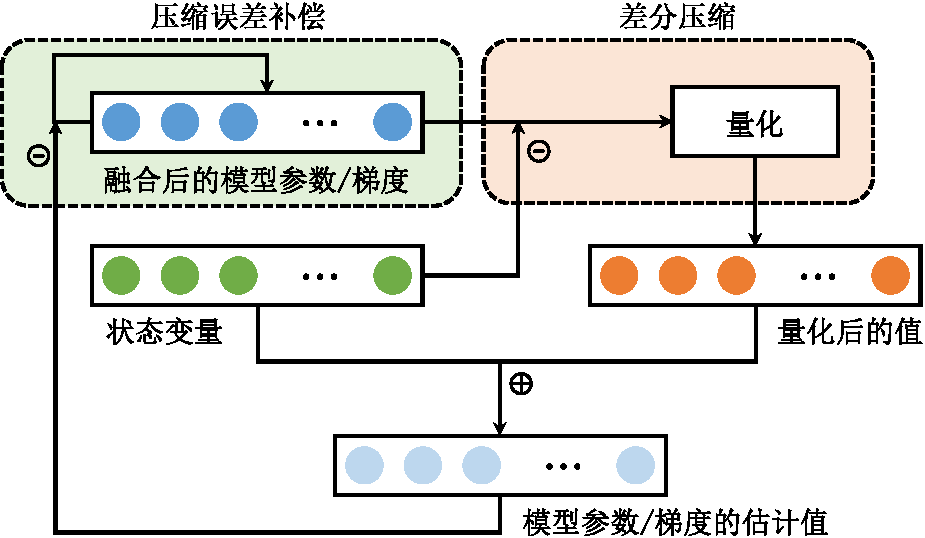
\includegraphics[width=0.7\linewidth]{figure/chapter4/fig4-2-error-quantize.pdf}
    \caption{\label{fig:Fig4-2}差分压缩与压缩误差补偿设计}
\end{figure}

进一步地，考虑在实际分布式深度学习任务的训练中，拓扑中不同边上的可用带宽可能不同，因此引入带宽矩阵$B$对算法进行改进。给定如下带宽矩阵，首先计算单位带宽$b_{unit}=\underset{i,j\in \left\{ 1,...,n \right\}}{\min}\,\,b_{ij}$。然后每个节点$i$计算其每条出边的带宽与单位带宽的比值$\frac{b_{ij}}{b_{unit}},\ j=1,...,n$，并找到满足$2^{m_{ij}}\leqslant \frac{b_{ij}}{b_{unit}}$的最大的$m_{ij}$。接下来根据设定的量化比特数$\mathrm{b}$，调整边$\left\{ i,j \right\}$上的量化比特数为$\mathrm{b}\times 2^{m_{ij}}$，并在进行通信前，根据对应的量化比特数对数据进行量化。通过引入如上改进，提高了高带宽边上的量化比特数，减小了对应的压缩误差，从而降低了量化对模型精度的影响。此外，上述改进方式能够使不同边上的通信时间尽量保持一致，而不会增加整体的通信时间，从而提高了资源的利用率。
\begin{equation}
    \label{tab:equ-4-12}
    B=\left[ \begin{matrix}
        b_{11}&		b_{12}&		\cdots&		b_{1n}\\
        b_{21}&		b_{22}&		\cdots&		b_{2n}\\
        \vdots&		\vdots&		\ddots&		\vdots\\
        b_{n1}&		b_{n2}&		\cdots&		b_{nn}\\
    \end{matrix} \right] 
\end{equation}

结合差分压缩、压缩误差补偿以及带宽自适应策略，本节提出的BA-QDSGD算法和BA-QDSGT算法的伪代码如\autoref{Algorithm-BA-QDSGD}和\autoref{Algorithm-BA-QDSGT}所示。

\begin{center}
    % \begin{minipage}{8.5cm}
    \begin{algorithm}[!htbp]
            \caption{节点$i$上的BA-QDSGD算法的伪代码} 
        %   \small
            \label{Algorithm-BA-QDSGD} 
            \begin{algorithmic}[1]
            \REQUIRE{模型参数初始值$\boldsymbol{x}_{i,0}$，状态变量初始值$H_{i,x,0}=\mathbf{0}$，参数$\left( \alpha ,\eta \right) $，步长$\gamma$，权重矩阵$W$，带宽矩阵$B$，量化比特数$\mathrm{b}$，迭代次数$K$}；
            \ENSURE{所有节点模型参数的平均值$\frac{1}{n}\sum_{i=1}^n{\boldsymbol{x}_{i,K}}$}；
            \STATE 初始化参数状态变量的加权平均值：$H_{i,x,w,0}=\sum_{j=1}^n{W_{ij}}H_{j,x,0}=\mathbf{0}$；
            \FOR{$k=0,1,...,K-1$}
                \STATE 根据带宽矩阵和量化比特数对参数进行差分压缩：\\\begin{center}$Q_{i,j,x,k}=compress\left( \boldsymbol{x}_{i,k}-H_{i,x,k},B,\mathrm{b} \right) ,\ j\in \mathcal{N} _{i}^{out} $；\end{center}
                \STATE 计算参数估计值：$\hat{\boldsymbol{x}}_{i,k}=H_{i,x,k}+Q_{i,i,x,k}$；
                \STATE 利用参数同步拓扑对压缩后的值进行通信，并将加权平均值与$H_{i,x,w,k}$求和得到$\hat{\boldsymbol{x}}_{i,w,k}$：\\\begin{center}$\hat{\boldsymbol{x}}_{i,w,k}=H_{i,x,w,k}+\sum_{j=1}^n{W_{ij}}Q_{j,i,x,k}$；\end{center}
                \STATE 更新参数对应的状态变量：\\\begin{center}$H_{i,x,k+1}=\alpha H_{i,x,k}+\left( 1-\alpha \right) \hat{\boldsymbol{x}}_{i,k},$\\$H_{i,x,w,k+1}=\alpha H_{i,x,w,k}+\left( 1-\alpha \right) \hat{\boldsymbol{x}}_{i,w,k}$；\end{center}
                \STATE 更新参数：$\boldsymbol{x}_{i,k+1}=\boldsymbol{x}_{i,k}-\eta \left( \hat{\boldsymbol{x}}_{i,k}-\hat{\boldsymbol{x}}_{i,w,k} \right) -\gamma \nabla f_i\left( \boldsymbol{x}_{i,k} \right) $。
            \ENDFOR            
            \end{algorithmic}
    \end{algorithm}
    % \end{minipage}
\end{center}


\begin{center}
    % \begin{minipage}{8.5cm}
    \begin{algorithm}[!htbp]
            \caption{节点$i$上的BA-QDSGT算法的伪代码} 
        %   \small
            \label{Algorithm-BA-QDSGT} 
            \begin{algorithmic}[1]
            \REQUIRE{模型参数初始值$\boldsymbol{x}_{i,0}$，辅助变量初始值$\boldsymbol{y}_{i,0}=\nabla f_i\left( \boldsymbol{x}_{i,0} \right) $，状态变量初始值$H_{i,x,0}=\mathbf{0}$和$H_{i,y,0}=\mathbf{0}$，参数$\left( \alpha ,\eta \right) $，步长$\gamma$，权重矩阵$W$，带宽矩阵$B$，量化比特数$\mathrm{b}$，迭代次数$K$}；
            \ENSURE{所有节点模型参数的平均值$\frac{1}{n}\sum_{i=1}^n{\boldsymbol{x}_{i,K}}$}；
            \STATE 初始化参数状态变量的加权平均值：$H_{i,x,w,0}=\sum_{j=1}^n{W_{ij}}H_{j,x,0}=\mathbf{0}$；
            \STATE 初始化梯度状态变量的加权平均值：$H_{i,y,w,0}=\sum_{j=1}^n{W_{ij}}H_{j,y,0}=\mathbf{0}$；
            \FOR{$k=0,1,...,K-1$}
                \STATE 根据带宽矩阵和量化比特数对参数进行差分压缩：\\\begin{center}$Q_{i,j,x,k}=compress\left( \boldsymbol{x}_{i,k}-H_{i,x,k},B,\mathrm{b} \right) ,\ j\in \mathcal{N} _{i}^{out} $；\end{center}
                \STATE 计算参数估计值：$\hat{\boldsymbol{x}}_{i,k}=H_{i,x,k}+Q_{i,i,x,k}$；
                \STATE 利用参数同步拓扑对压缩后的值进行通信，并将加权平均值与$H_{i,x,w,k}$求和得到$\hat{\boldsymbol{x}}_{i,w,k}$：$\hat{\boldsymbol{x}}_{i,w,k}=H_{i,x,w,k}+\sum_{j=1}^n{W_{ij}}Q_{j,i,x,k}$；
                \STATE 更新参数对应的状态变量：\\\begin{center}$H_{i,x,k+1}=\alpha H_{i,x,k}+\left( 1-\alpha \right) \hat{\boldsymbol{x}}_{i,k},$\\$H_{i,x,w,k+1}=\alpha H_{i,x,w,k}+\left( 1-\alpha \right) \hat{\boldsymbol{x}}_{i,w,k}$；\end{center}
                \STATE 更新参数：$\boldsymbol{x}_{i,k+1}=\boldsymbol{x}_{i,k}-\eta \left( \hat{\boldsymbol{x}}_{i,k}-\hat{\boldsymbol{x}}_{i,w,k} \right) -\gamma \boldsymbol{y}_{i,k}$；

                \STATE 根据带宽矩阵和量化比特数对梯度进行差分压缩：\\\begin{center}$Q_{i,j,y,k}=compress\left( \boldsymbol{y}_{i,k}-H_{i,y,k},B,\mathrm{b} \right) ,\ j\in \mathcal{N} _{i}^{out} $；\end{center}
                \STATE 计算梯度估计值：$\hat{\boldsymbol{y}}_{i,k}=H_{i,y,k}+Q_{i,i,y,k}$；
                \STATE 利用参数同步拓扑对压缩后的值进行通信，并将加权平均值与$H_{i,y,w,k}$求和得到$\hat{\boldsymbol{y}}_{i,w,k}$：$\hat{\boldsymbol{y}}_{i,w,k}=H_{i,y,w,k}+\sum_{j=1}^n{W_{ij}}Q_{j,i,y,k}$；
                \STATE 更新梯度对应的状态变量：\\\begin{center}$H_{i,y,k+1}=\alpha H_{i,y,k}+\left( 1-\alpha \right) \hat{\boldsymbol{y}}_{i,k},$\\$H_{i,y,w,k+1}=\alpha H_{i,y,w,k}+\left( 1-\alpha \right) \hat{\boldsymbol{y}}_{i,w,k}$；\end{center}
                \STATE 更新梯度：$\boldsymbol{y}_{i,k+1}=\boldsymbol{y}_{i,k}-\eta \left( \hat{\boldsymbol{y}}_{i,k}-\hat{\boldsymbol{y}}_{i,w,k} \right) +\nabla f_i\left( \boldsymbol{x}_{i,k+1} \right) -\nabla f_i\left( \boldsymbol{x}_{i,k} \right) $。
            \ENDFOR            
            \end{algorithmic}
    \end{algorithm}
    % \end{minipage}
\end{center}

算法中的$compress$函数为\autoref{tab:equ-4-8}的压缩函数，$H_{i,x}$和$H_{i,y}$是节点$i$用于实现差分压缩而引入的状态变量，$Q_{i,j,x}$和$Q_{i,j,y}$是根据边$\left\{ i,j \right\} $上的量化比特数进行差分压缩得到的结果，$\mathcal{N} _{i}^{out}$是节点$i$的出邻居。随着算法的运行，$H_{i,x}$和$H_{i,y}$最终将分别收敛到参数$\boldsymbol{x}_i$和辅助变量$\boldsymbol{y}_i$，从而使得由差分压缩导致的误差消失。此外，将BA-QDSGT算法中$n$个节点的参数更新公式合并可以得到：
\begin{equation}
    \label{tab:equ-4-13}
    \boldsymbol{x}_{k+1}=\boldsymbol{x}_k-\eta \left( I-W \right) \hat{\boldsymbol{x}}_k-\gamma \boldsymbol{y}_k.
\end{equation}
对于BA-QDSGD算法，式中的$\boldsymbol{y}_k$替换为$\nabla f\left( \boldsymbol{x}_k \right) $。令参数压缩误差$\boldsymbol{e}_{x,k}=\boldsymbol{x}_k-\hat{\boldsymbol{x}}_k$，则有：
\begin{equation}
    \label{tab:equ-4-14}
    \begin{aligned}
        \boldsymbol{x}_{k+1}&=\boldsymbol{x}_k-\eta \left( I-W \right) \left( \boldsymbol{x}_k-\boldsymbol{e}_{x,k} \right) -\gamma \boldsymbol{y}_k
        \\
        &=\left[ \left( 1-\eta \right) +\eta W \right] \boldsymbol{x}_k-\gamma \boldsymbol{y}_k+\eta \left( I-W \right) \boldsymbol{e}_{x,k}.
    \end{aligned}
\end{equation}
式中的最后一项$\eta \left( I-W \right) \boldsymbol{e}_{x,k}$说明每个节点会将其压缩误差在本地累加，同时随着参数发送给其他节点，从而实现全局压缩误差补偿。同样地，辅助变量$\boldsymbol{y}$也会实现压缩误差补偿。

BA-QDSGT算法的另一个比较重要的特点是保证了梯度跟踪方法的有效性，将$n$个节点的梯度更新公式合并可以得到：
\begin{equation}
    \label{tab:equ-4-15}
    \boldsymbol{y}_{k+1}=\boldsymbol{y}_k-\eta \left( I-W \right) \hat{\boldsymbol{y}}_k+\nabla f\left( \boldsymbol{x}_{k+1} \right) -\nabla f\left( \boldsymbol{x}_k \right) .
\end{equation}
对等式两边同时左乘$\mathbf{1}^T$后，得到：
\begin{equation}
    \label{tab:equ-4-16}
    \begin{aligned}
        1^T\boldsymbol{y}_{k+1}&=1^T\left( \boldsymbol{y}_k-\eta \left( I-W \right) \hat{\boldsymbol{y}}_k+\nabla f\left( \boldsymbol{x}_{k+1} \right) -\nabla f\left( \boldsymbol{x}_k \right) \right) 
        \\
        &=1^T\boldsymbol{y}_k+1^T\nabla f\left( \boldsymbol{x}_{k+1} \right) -1^T\nabla f\left( \boldsymbol{x}_k \right) 
        \\
        &=1^T\nabla f\left( \boldsymbol{x}_{k+1} \right) .
    \end{aligned}
\end{equation}
这说明当辅助变量收敛到一致时，所有节点都能够跟踪全局平均梯度，从而保证本地参数朝相同方向更新。

\section{算力分析}
本节对提出的BA-QDSGD算法和BA-QDSGT算法的有效性进行验证，并与现有的分布式训练算法进行对比分析。所有实验都是在同一个硬件系统上完成的，该系统配备了2个Intel Xeon Gold 6226R处理器和8个NVIDIA GeForce RTX 2080 Ti，每个GPU有11GB显存。该硬件系统采用\autoref{fig:Fig2-4}所示的标准服务器架构。本节的实验使用pytorch实现。

\subsection{实验设置}
本节选用Cifar10数据集和ResNet-18模型进行分布式深度学习实验。在训练开始之前，每个节点从每个类别的训练数据中随机采样相同数量的样本构成本地训练数据集。实验的超参数中批大小设置为32（每个节点），学习率设置为0.05，动量因子设置为0.9，权重衰减设置为0.0001，训练周期数设置为100。另外，BA-QDSGD算法和BA-QDSGT算法中的参数$\alpha$设置为0.5，$\eta$设置为1。

实验中采用的参数同步拓扑基于第三章的优化方法得到，根据第二章的测试结果，服务器内部三种物理链路的带宽比为$e_{PIX}:e_{NODE}:e_{SYS}=9.76GB/s:11.05GB/s:11.03GB/s$，令边的数目分别为10和16，基于\autoref{Algorithm-T-ADMM}得到如\autoref{fig:Fig4-3}所示的两个参数同步拓扑。本节的分布式深度学习实验将在这两个参数同步拓扑上进行。

\begin{figure}[!htbp]
    \centering
    \subfigure[$r=10$]{
        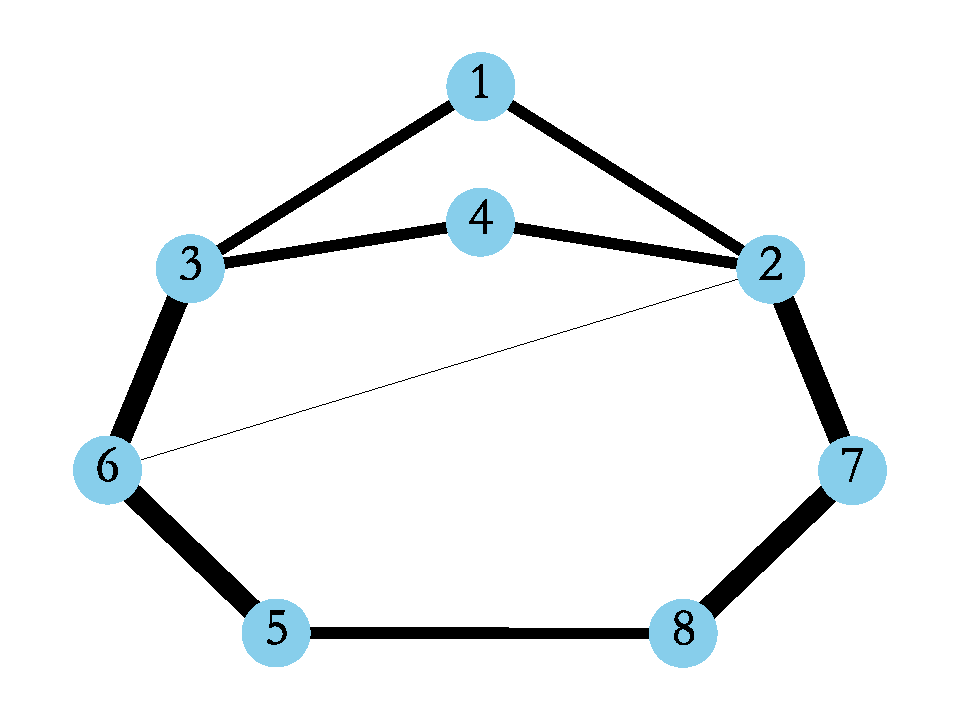
\includegraphics[width=0.48\linewidth]{figure/chapter4/fig4-3-topo1.pdf}
    }
    \subfigure[$r=16$]{
        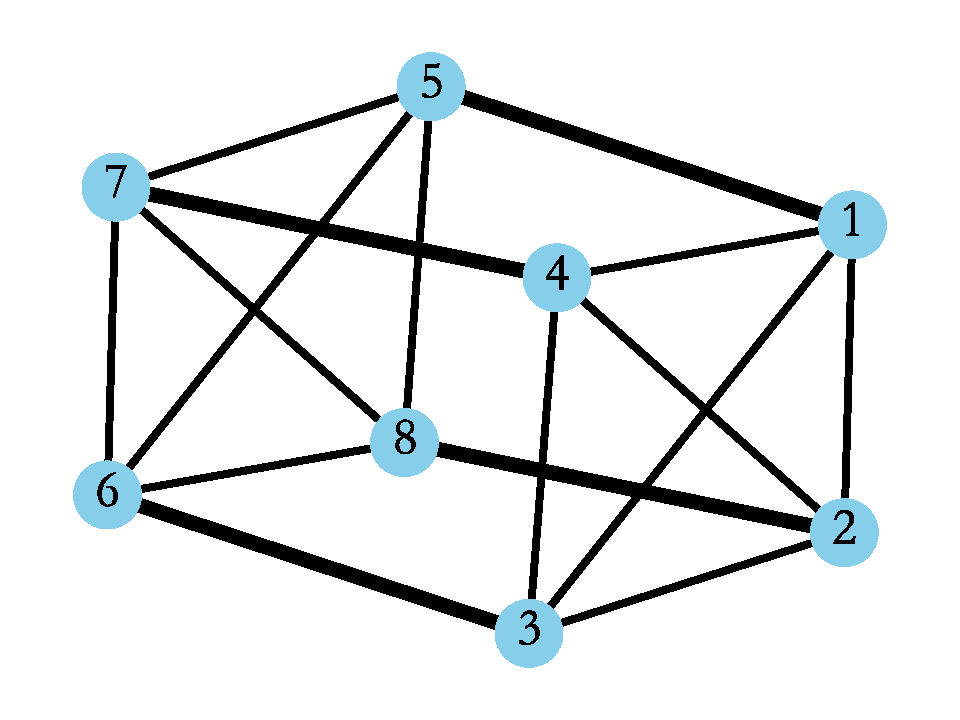
\includegraphics[width=0.48\linewidth]{figure/chapter4/fig4-3-topo2.pdf}
    }
    \caption{\label{fig:Fig4-3}分布式深度学习实验采用的参数同步拓扑}
\end{figure}

本节对比的分布式训练算法包括DSGD算法、DSGT算法、Choco-SGD算法\cite{koloskova2019decentralized}和C-GT算法\cite{li2021compressed}。其中Choco-SGD算法和C-GT算法分别对DSGD算法和DSGT算法引入了差分压缩和压缩误差补偿策略。

\subsection{实验结果与分析}
本小节首先在两种参数同步拓扑上验证了本章提出的BA-QDSGD算法和BA-QDSGT算法的收敛性：将QDSG算法、Choco-SGD算法和BA-QDSGD算法进行对比，将QDST算法、C-GT算法和BA-QDSGT算法进行对比，令量化比特数$\mathrm{b}$分别等于2、4和8，




从以下几个方面设计实验以验证本章提出的BA-QDSGD算法和BA-QDSGT算法的有效性：实验1验证了不同量化程度下BA-QDSGD算法和BA-QDSGT算法的收敛性；实验2

\section{本章小结}